\chapter{Background}
\label{c:background}

In this chapter, we review important properties of several technologies or terms that are used in FileFarm.

% Cloud Computing
\section{Cloud Computing}
\label{s:cloudcomputing}

Cloud computing is a model describing the relationship between computing resources, service providers and consumers over network connections. In this model, service providers make efforts to offer consumers a convenient, reliable and on-demand way of accessing computing resources. The providers' computing resources are normally pooled to serve multiple consumers using a multi-tenant way with different physical and virtual resources dynamically assigned and reassigned according to consumer's demand. From consumer's point of view, the capabilities available often appear to be unlimited and can be elastically provisioned and released in any amount as long as they need. Furthermore, the resource usage can usually be measured with certain metrics (e.g., storage, processing, bandwidth and active user accounts) and be reported to both provider and consumers transparently. Based on a signed contract, provider then charges consumers in regular basis according to resource usage.\cite{mell2011nist}

With cloud computing technology, enterprises obtain an easy way toward computing outsourcing, in a sense that they no longer need to commit a large amount of capital on hardware and software to build their own IT infrastructure before product launch. Instead, they can rapidly allocate just-enough computing power and storage space as they need with minimal management overhead. They can also elastically expand or reduce the amount of allocated resources based on changes of business scale. Due to the flexibility and reliability, cloud computing has given rise to a paradigm shift in how computing services are deployed and delivered.\cite{6123700}

% Cloud Storage Service
\section{Cloud Storage Service}
\label{s:cloudstorageservice}

Among all types of cloud computing services, storage is nearly the most fundamental one that many others are built upon. To offer a reliable, widely-available cloud storage service, providers build infrastructure and data centers spanning all over the world. Besides hardware deployment, providers also develop software to take care of aspects such as access management, resource routing, replication schema, error correction code, load-balancing... All efforts done by providers contribute to a single purpose: to provide consumer with a robust, easy-to-access online disk space. From consumer's point of view, the storage service seems much simpler. To access the storage service, consumers connect to provider's servers using a pre-defined API. The allowed API operations should at least include POST, GET, DELETE, by which consumers can upload, download and remove data, respectively.

Cloud storage service is a mature technology and business that changes the way data are stored and accessed. Among all existing cloud storage services, Amazon AWS S3\cite{awss3}, Google Cloud Storage\cite{googlecloudstorage}, Microsoft Azure\cite{msazurestorage} are 3 successful instances. Depending on usage size, access rate and service-level agreement, a storage provider may provide various storage service products. The pricing schema of cloud storage services usually involves 2 major usage factors: (1) \textit{static storage} (2) \textit{data transfer}. The former one is the fee of storing data statically, charged in per GB/month basis, whereas the latter one charges consumers every GB of data downloaded from the cloud (upload traffics are usually for free). The 2 factors collectively account for the primary part of storage fee.

Cloud storage services have successfully relieve individuals or enterprise consumers from affording the high cost of maintaining their own storage systems. Due to the economies of scale, cost of cloud storage solution is usually much lower than that of building a storage infrastructure with same level of reliability on consumers' own. Thus, cloud storage has gradually dominated the choice of enterprises over other storage options\cite{storagetrends2018}.

% Cloud-of-Clouds
\section{Cloud-of-Clouds}
\label{s:cloudofclouds}

Although cloud computing provides benefits in terms of low cost, elasticity and reliability, ensuring security of data stored on clouds remains an unsolved problem, as consumers often store critical and sensitive data on the services offered by a third-party provider which may be untrusted. To solve this issue, researchers have moved forward to  a new research domain\cite{aizain2012multiclouds}. "Cloud-of-clouds", or "multi-clouds", "interclouds" is an area of research aiming to build a service on multiple clouds and avoid dependence or data leakage on any of them. The term was firstly introduced by Vukolic\cite{vukolic2010byzantine}. Multiple designs have been proposed at around the same time\cite{bowers2009hail},\cite{abu2010racs},\cite{cachin2010dependable},\cite{bessani2013depsky}. The research in this area has often been formulated as a Byzantine fault tolerance problem\cite{lamport1982byzantine}, in the sense that any faults occurring to a cloud may lead to misbehavior of it, while the system is designed to tolerate certain level of concurrent cloud failures. Besides, approaches of solving the single-cloud problem often integrate certain means of coding techniques that not only add redundancy to data, but also make sure that a file is not view-able or recoverable from any single cloud. This way, risks of malicious insider or single cloud service failure can be reduced significantly.

% Hybrid Cloud
\section{Hybrid Cloud}
\label{s:hybridcloud}

Hybrid cloud is a specialized branch of cloud-of-clouds research. In the settings of hybrid cloud, part of the enterprises' service is held by their own servers. Integration of both public clouds and private servers contributes to a more rapid and robust service. Such hybrid design is actually a more practical and feasible deployment option for most enterprises. As mentioned above, public clouds bring benefits of reliability, flexibility and cost-efficiency; however, they cannot provide certain benefits of servers in private network, such as security, low-latency and full control over data. With proper design, hybrid cloud systems have the potential of bringing the best of both public clouds and private premises, while minimizing the disadvantages of them. A cloud storage example under this topic is: \textit{Hybris}\cite{dobre2014hybris}.

% Peer-to-Peer Systems
\section{Peer-to-Peer Systems}
\label{s:peertopeersystems}

Peer-to-Peer is a computing or networking architecture in which each participant, called \textit{node} or \textit{peer}, shares equal responsibility of maintaining the dedicated service. In a P2P system, peers are equally-privileged and follow the same protocol to negotiate with each other, without a centralized coordinator over them. Instead of aggregating storage and computing power to a single serving machine, each peer in a P2P system contributes part of its resources to the network, and requires the resources it wants from other peers in return. A properly-designed P2P system will eventually meet all peers' need. Because of the distributed architecture, P2P model does not suffer from single-point-of-failure problem, which means such systems are generally robust to frequent churning of peers, network topology changes, or failures occurring to part of the network. Besides, since peers serve needs for each other without a centralized channel, P2P systems tend to have better throughput and service capability comparing with traditional client-server models. However, since there are no central node in a P2P network, a peer needs to coordinate with other peers on its own and achieve a consistent state of consensus with others, in terms of routing information, content location, status of other peers, ... This brings extra computational and timing overhead to peer applications. Due to this, P2P protocols are usually more difficult to design then client-server ones, and some P2P systems are suffering from efficiency and scalability issues. In spite of the difficulty, P2P systems have still found their popularity in many application domains, with content sharing being the origin of the whole concept and the most successful one so far. \textit{Napster}\cite{napster}, \textit{BitTorrent}\cite{bittorrent}, \textit{eMule}\cite{emule}, \textit{aMule}\cite{amule} are some successful P2P content sharing applications.

% Distributed Hash Table
\section{Distributed Hash Table}
\label{s:distributedhashtable}

How to search for data over a fully-distributed network has always been a research topic drawing high attention. Of all kinds of means proposed, distributed hash table (DHT) is the most popular category due to its high efficiency. Generally speaking, DHT is a content-addressed approach in which each piece of data is assigned with a \textit{key} defined as its hash value. The piece of data is then stored in the distributed network according to its \textit{key}. Thus, the locations where a given piece of data should be stored are defined by its content. This introduces de-duplication feature for such systems since same content will always be stored on same set of nodes. Besides, the dispersal and randomness properties of hash function also enable DHT-based systems to be designed in a load-balancing way. In P2P applications, DHTs are often implemented as an overlay or infrastructure that more complex services can be built upon. Such applications then inherit the desired features of their underlying DHTs. A DHT protocol also defines how to lookup and retrieve data from the network. Efficiency of the lookup processes has a direct impact on performance and usability of systems based on the DHT. Most of the widely-used DHTs have logarithm-time guarantee on worst-case lookup length. Chord\cite{stoica2001chord}, Kademlia\cite{maymounkov2002kademlia}, Pastry\cite{rowstron2001pastry}, Tapestry\cite{zhao2004tapestry} are some well-known DHT protocols, to name a few.

% Kademlia
\section{Kademlia}
\label{s:kademlia}
Kademlia\cite{maymounkov2002kademlia} is a popular structured DHT protocol applied on a number of modern P2P applications including BitTorrent\cite{bittorrent}, Ethereum\cite{ethereum}, IPFS\cite{ipfs} and Storij\cite{storij}, ... The wide adoption of Kademlia can be attributed to several desired properties it provides. We categorize these properties into 3 aspects: \textit{load balancing}, \textit{efficient search} and \textit{redundancy maintenance}.

\subsection{Load Balancing}
\label{ss:loadbalancing}
In a Kademlia network, storage load of composing nodes are roughly balanced. This property is assured by the underlying ID assignment and content-addressable designs. In Kademlia, each node is assigned with a randomly-generated 160-bit ID when it starts up. Besides, each data chunk to be stored in the network is identified by its SHA-1 hash value (aka. \textit{key}), which is also 160-bit in length. Since node IDs and keys share exactly the same format, they are also able to share the same \textit{distance metric}. Given 2 identifiers (node ID or key), $x$ and $y$, the distance between them is defined as their bit-wise exclusive or (XOR) interpreted as an integer, $\delta(x,y)=x \oplus y$. With distance metric defined, Kademlia further regulates that each piece of data should be stored at the \textit{$K$ nodes with ID closest to the its key}, where $K$ is a system-wise redundancy parameter. Due to the randomness of node IDs and keys, data pieces are uniformly distributed over the storage nodes, with each node's load expected to be balanced.

\subsection{Efficient Search}
\label{ss:efficientsearch}

Kademlia provides an efficient way to search for a piece of data in a P2P network given its \textit{key}. Like many other DHT alternatives, it takes no more than $\lceil log(n) \rceil + c$ iterated queries to lookup any target in a Kademlia network. In this subsection, we explain the lookup mechanisms of Kademlia in detail.

As described in \ref{ss:loadbalancing}, a piece of data should be stored on the $K$ nodes with ID closest to the its key. These $K$ nodes are uniquely defined by the XOR distance metric, and can be found by lookup procedures specified in Kademlia protocol. To know how these procedures work, we first take a look at how routing information is kept on each node. Kademlia's ID space can be represented as a binary tree (also called \textit{trie}) of height 160, with each ID representing a leaf node in the trie. Figure \ref{fig:buckettrie} shows an example of the trie in a small Kademlia network where ID length $d = 4$. The leaves of this trie represent all possible node IDs in this network. Given an ID $x$, the trie can be partitioned into $d$ subtrees as follows:

\begin{center}
  $D_{i}(x) = {y: \delta(x,y) \in [2^{i-1}, 2^{i}]}, i = 1, 2, ..., d$
\end{center}

Notice that IDs in each subtree share the same prefix, where the last bit of the prefix indicates the most significant difference bit between $x$ and IDs in the corresponding subtree, which determines the distance from these IDs to $x$. Thus, the longer the prefix is, the closer the IDs are to $x$. For instance, IDs in $D_{2}(x)$ share prefix $101$, which indicates that all IDs in $D_{2}(x)$ share the same first 2 bits with $x$ while their third bit is different from $x$. Thus, distance between x and IDs in $D_{2}(x)$ ranges from $2^{1}$ to $2^{2}-1$. From this point of view, it is clear that this partition splits the entire ID space into $d$ disjoint parts according to the XOR distance metric.

\begin{figure}[hbt]
  \centering
    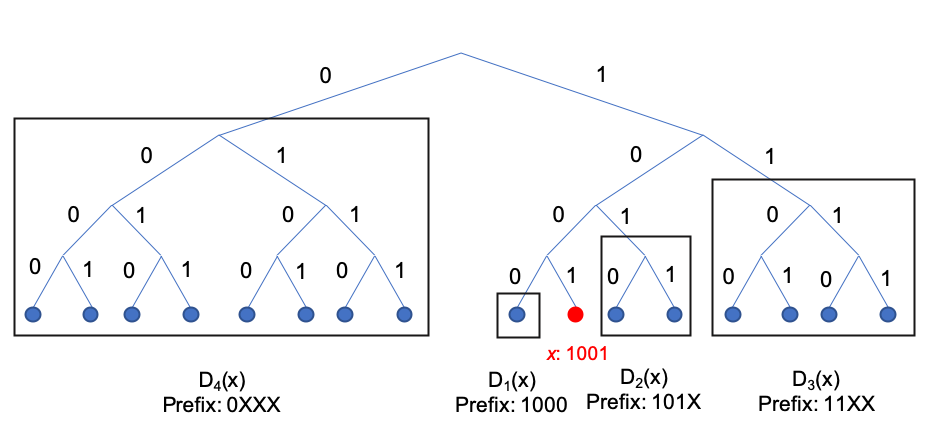
\includegraphics[width=13cm]{figures/bucket_trie.png}
    \caption{An example of Kademlia's Trie with ID length = 4}
    \label{fig:buckettrie}
\end{figure}

In Kademlia, a node with ID $x$ maintains a routing table that keeps at most $K$ records of peers for each subtrees in $D_{1}(x), D_{2}(x), ..., D_{d}(x)$. With this routing table, the node is acknowledged of peers' contact information from a wide range of distance.

Before explaining details of lookup procedures, we define 2 types of RPCs (Remote Procedure Call) used by Kademlia nodes to communicate with each other:
\begin{itemize}
  \item \textit{FIND\_NODE}:
  \begin{itemize}
    \item \textbf{Input}: a 160-bit TARGET\_ID
    \item \textbf{Output}: $K$ triples of \textit{<IP address, UDP port, Node ID>} known by the receiver with Node IDs closest to TARGET\_ID
  \end{itemize}
  \item \textit{FIND\_VALUE}
  \begin{itemize}
    \item \textbf{Input}: a 160-bit TARGET\_KEY
    \item \textbf{Output}: 
    \begin{itemize}
      \item The data chunk with key being TARGET\_KEY; if the receiver does store the data chunk with key being TARGET\_KEY
      \item $K$ triples of \textit{<IP address, UDP port, Node ID>} known by the receiver which are closest to TARGET\_KEY; otherwise
    \end{itemize}
  \end{itemize}
\end{itemize}

\noindent Now we describe the lookup procedures. In Kademlia, there are 2 types of lookup:
\begin{itemize}
  \item \textit{NODE\_LOOKUP}: to find the $K$ nodes in the network with ID closest to a target ID
  \item \textit{VALUE\_LOOKUP}: to find the content corresponding to a target key
\end{itemize}

\noindent \textbf{Algorithm \textit{NODE\_LOOKUP:}}
\begin{itemize}
  \item \textbf{Input}: a 160-bit TARGET\_ID, $K$ triples of \textit{<IP address, UDP port, Node ID>} known by the initializer with Node IDs closest to TARGET\_ID
  \item \textbf{Output}: $K$ triples of \textit{<IP address, UDP port, Node ID>} in the network with Node IDs closest to TARGET\_ID
\end{itemize}
\begin{enumerate}[label=(\roman*)]
  \item The initializer puts the $K$ closest nodes it knows into a lookup-memory.
  \item The initializer picks $\alpha$ nodes from the lookup-memory, where $\alpha$ is a system-wide concurrency parameter, such as 3.
  \item The initializer sends parallel, asynchronous FIND\_NODE RPCs to these $\alpha$ nodes and expect to receive $K$ closest node records known by each of them.
  \item When receiving a FIND\_NODE response containing k node candidates, the initializer updates these candidates to the lookup-memory and leaves only $K$ closest ones. Then the initializer picks $\alpha$ un-queried nodes from the lookup-memory and sends FIND\_NODE RPCs to them.
  \item If a round of FIND\_NODE fails to return closer nodes than the ones in the lookup-memory, the initializer sends FIND\_NODEs to all un-queried nodes in the lookup-memory.
  \item The NODE\_LOOKUP procedure terminates when the initializer receives all responses. Now the $K$ nodes in lookup-memory are the $K$ closest ones to TARGET\_ID over the network and should be returned.
\end{enumerate}

\noindent \textbf{Algorithm \textit{VALUE\_LOOKUP:}}
\begin{itemize}
  \item \textbf{Input}: a 160-bit TARGET\_KEY, $K$ triples of \textit{<IP address, UDP port, Node ID>} known by the initializer with Node IDs closest to TARGET\_KEY
  \item \textbf{Output}:
  \begin{itemize}
    \item The TARGET\_CHUNK with key being TARGET\_KEY; if TARGET\_CHUNK exists in the network
    \item $K$ triples of \textit{<IP address, UDP port, Node ID>} in the network which are closest to TARGET\_KEY; otherwise
  \end{itemize}
\end{itemize}
\begin{enumerate}[label=(\roman*)]
  \item The initializer puts the $K$ closest nodes it knows into a lookup-memory.
  \item The initializer picks $\alpha$ nodes from the lookup-memory, where $\alpha$ is a system-wide concurrency parameter, such as 3.
  \item The initializer sends parallel, asynchronous FIND\_VALUE RPCs to these $\alpha$ nodes.
  \item When receiving a FIND\_VALUE response containing TARGET\_CHUNK, the procedure ends by returning TARGET\_CHUNK.
  \item When receiving a FIND\_VALUE response containing $K$ node candidates, the initializer updates these candidates to the lookup-memory and leaves only $K$ closest ones. Then the initializer picks $\alpha$ un-queried nodes from the lookup memory and sends FIND\_VALUE RPCs to them.
  \item If a round of FIND\_VALUE fails to return closer nodes than the ones in the lookup-memory, the initializer sends FIND\_VALUEs to all un-queried nodes in the lookup-memory.
  \item The VALUE\_LOOKUP procedure terminates when the initializer receives all responses. In this case, the initializer fails to find TARGET\_CHUNK, and the $K$ nodes in the lookup memory closest to TARGET\_KEY should be returned.
\end{enumerate}

Now we want to discuss the efficiency of NODE\_LOOKUP and VALUE\_LOOKUP procedures. According to the sketch of proof in \cite{maymounkov2002kademlia}, NODE\_LOOKUP in a Kademlia network will finish in $\lceil log(n) \rceil + c$ steps for some small constant of $c$, where $n$ is network size, i.e., number of nodes in the network. This gives an rough upper bound for NODE\_LOOKUP efficiency.

Different from NODE\_LOOKUP, the VALUE\_LOOKUP procedure finishes immediately when the target value is found. Thus, VALUE\_LOOKUP procedure only needs to reach any one of the $K$ closest nodes instead of finding all of them. According to Cai's analysis\cite{cai2013probabilistic}, it takes no more than $(1+O(1))\frac{log(n)}{H_{K}}$ steps for any node in a Kademlia network to locate any other node, where $H_K = \sum_{i=1}^{K} 1/i$. This upper bound also stands for VALUE\_LOOKUP, considering the fact that VALUE\_LOOKUP for the target key converges along the same path as NODE\_LOOKUP for the closest farmer, due to \textit{unidirectionality} of XOR distance metric: For any given point $x$ and distance $\Delta>0$, there is exactly one point $y$ such that $d(x,y)=\Delta$.

From the analysis above, we know that both NODE\_LOOKUP and VALUE\_LOOKUP procedures are guaranteed to be finished in logarithm steps, while VALUE\_LOOKUP takes a tighter bond with a factor of $H_K = \sum_{i=1}^{K} 1/i$, since only 1 copy of data is required to be found, and we can find it by reaching any of the $K$ storing nodes.

\subsection{Redundancy Maintenance}
\label{ss:redundancymaintenance}
Redundancy maintenance is another desired property provided by Kademlia. When a node churns off from the network, each of the data chunks it used to stored will lose one redundancy copy. Kademlia has a \textit{efficient key republishing} mechanism ensuring that each chunk will always have at least $K$ copies over the storage network.

The \textit{efficient key republishing} mechanism regularly checks if each data chunk is stored on the $K$ closest farmers. If any of the $K$ closest farmers does not store the chunk, a copy will be sent to it automatically. This assurance is provided by the design in which each farmer periodically attempts to \textit{republish} each chunk it stored to the other $K-1$ farmers who should store the same chunk. During the republishing period, if a farmer receives the republishing message of a chunk from other farmer, it assumes the message has also been sent to the other $K-1$ closest farmers and thus it should not republish it again during this period in order to reduce traffic. As long as the republishing interval of farmers are not exactly synchronized, there will only be exactly 1 republishing message for each chunk in each interval. However, the efficient key republishing mechanism has a considerable overhead. Within a \textit{republishing period}, each chunk induces one NODE\_LOOKUP followed by $K$ republishing messages. Choices of longer republishing period would mitigate the overhead while providing weaker guarantee on retrievability of files.

% Information Dispersal Algorithm
\section{Information Dispersal Algorithm}
\label{s:informationdispersalalgorithm}

Information Dispersal Algorithm (IDA)\cite{rabin1989efficient} is a computation schema of dispersing content of a file into smaller chunks and reconstructing the original file based on some of the chunks, where the dispersal and reconstruction process are computationally efficient. To be more precise, a $(p,q)$ IDA schema breaks a file $F$ into $p + q$ chunks of size $\frac{|F|}{p}$, such that $F$ can be reconstructed from any p chunks but not less. Figure \ref{fig:ida} shows an example of dispersing a file $F$ of size $|F|=16$ bytes with a $(4,2)$ schema. In the figure, each byte is represented as an integer from $[0, 255]$. The first step of IDA is to split the original file into $p=4$ chunks, with each chunk being a row of the matrix representing the entire file. After that, a randomly generated matrix $M$ of size $(p+q)\times p$ is being multiplied with the file matrix and the computation yields a matrix of size $(p+q)\times \frac{|F|}{p}$. Each row in the result matrix is a computed chunk that is supposed to be stored in a place different from others. To reconstruct the original file $F$, one needs to collect $p$ computed chunks and multiply the collected chunks with inverse matrix of concatenation of their corresponding rows in $M$. As long as the corresponding rows in $M$ are linearly independent, the original file can be reconstructed based on these $p$ collected chunks.

Due to its potential traits of security, load-balancing and fault tolerance design, Information Dispersal Algorithm is widely-used in distributed file storage and content sharing applications. Considering a distributed network of computers and workstations, files pre-processed with IDA are certainly hard to be reconstructed by nodes other than the uploader, since only the uploading node has the knowledge of dispersion keys and distribution of chunks in the network. Besides, in a distributed application, the stored chunks can be downloaded from different nodes in parallel, this boosts the downloading performance of large files.  Also, the $q$ factor in the IDA schema makes redundancy and tolerance in a fault-prone environment. These are reasons why IDA is suitable for distributed systems.

\begin{figure}[hbt]
\centering
  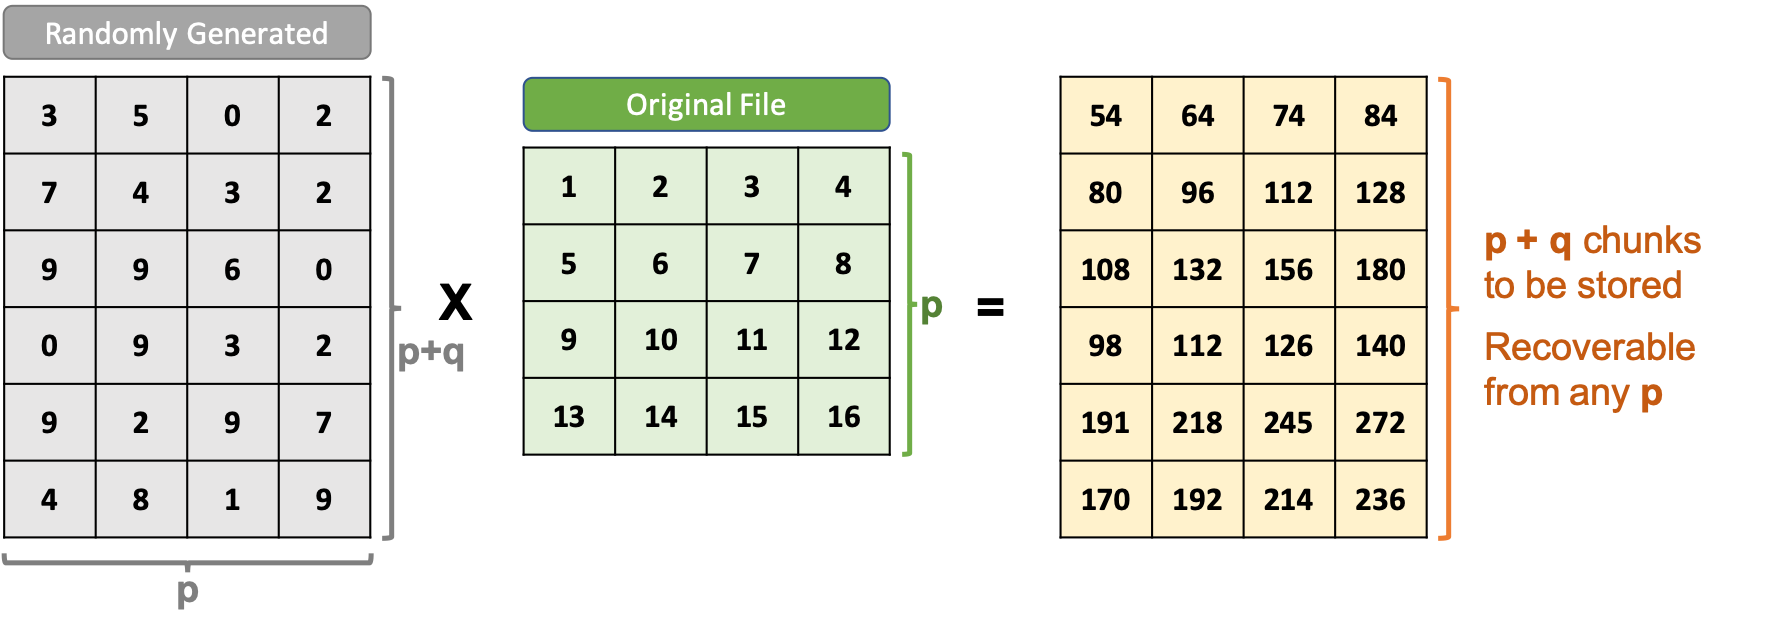
\includegraphics[width=13cm]{figures/ida.png}
  \caption{An example of IDA with schema $(p,q)=(4,2)$}
  \label{fig:ida}
\end{figure}

% Public Key Infrastructure
\section{Public Key Infrastructure}
\label{s:publickeyinfrastructure}

Public key infrastructure (PKI) is an infrastructure that enables entities to securely communicate over an insecure public network via cryptographic techniques of public-key encryption, digital signature and certificate-based authentication. From the perspective of cryptography, PKI is a reliable approach to bind public keys with respective identities. The binding process is facilitated by registration and issuance of digital certificates, which can be demonstrated by Figure \ref{fig:pki}: The whole process involves 3 parties: an entity providing service to users, an certificate authority (CA) and a user. To get a certificate, the entity needs to generate a certificate request (CSR) containing its public key first. It then sends the CSR to CA. With all means of verification, CA finally trusts the entity. CA then generates a certificate for the entity, which includes CA's digital signature signed with its private key. The certificate is then sent back to the entity and installed on its server machine. From now on, whenever a user sends a connection request to the entity, it responses with its certificate. The user then verifies this certificate by validating the CA's signature on the certificate. If the verification passes, the user will establish a secure connection with the entity encrypted by the entity's public key.

PKI is a general term involving policies of issuing, managing, and validating digital certificates. Inside this broad term, X.509\cite{rfc4158} is a majorly adopted standard defining the format of public key certificates, which is widely used in the Internet and is the fundamental technique implemented in TLS/SSL, the basis of HTTPS.

\begin{figure}[hbt]
\centering
  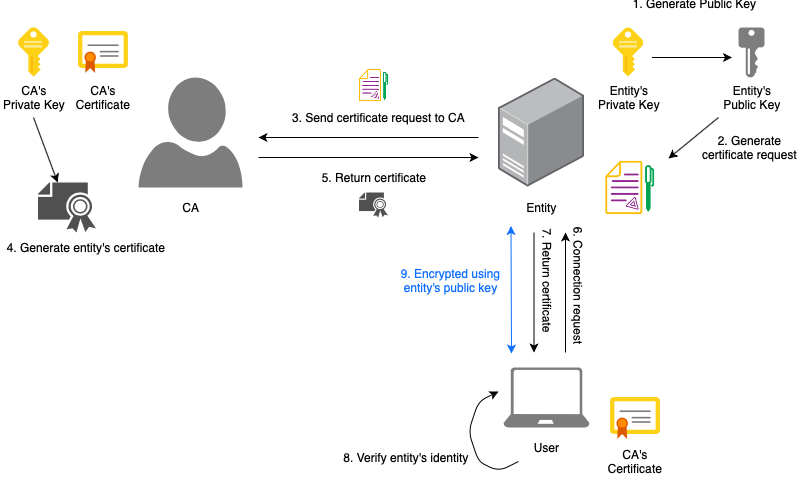
\includegraphics[width=14cm]{figures/pki.png}
  \caption{Procedure of certificate issuance and certificate-based authentication}
  \label{fig:pki}
\end{figure}